All the seismic measurements have been made possible with the dedication and help from a vast number of locals. To all the people (see also section \ref{Acknowledgements}) that have provided their expertise, time and assistance we would like to extend a sincere thank you. 

\pagebreak
\FloatBarrier
\subsubsection*{Germany - Black forest}
\begin{figure}[h]
\centering
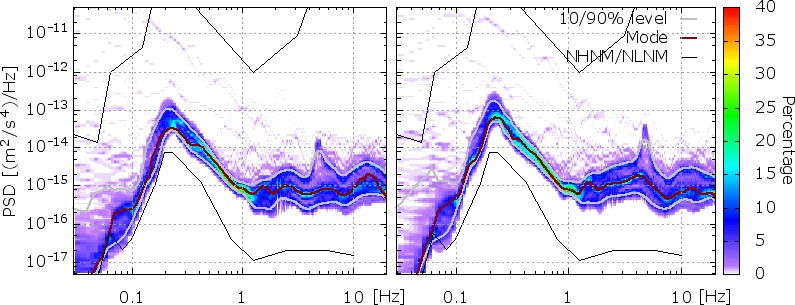
\includegraphics[width=\textwidth]{./Sec_SiteInfra/Figures/results/ZWald-A_multiplot1}
\caption{The horizontal component (left) and the vertical component (right) power spectral density plotted as a spectral variation from the Germany - Black forest site.}
\label{fig:ZWald-A_multiplot1}
\end{figure}\begin{figure}[h]
\centering
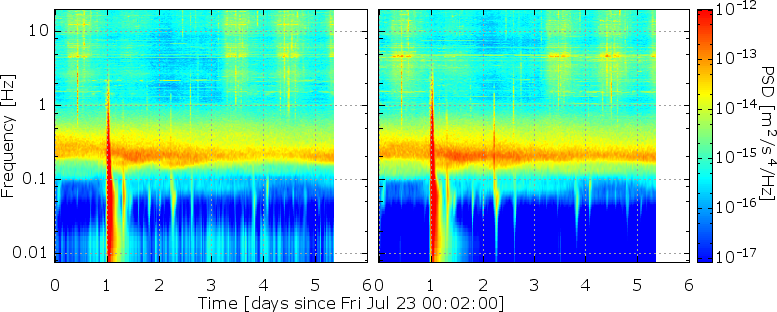
\includegraphics[width=\textwidth]{./Sec_SiteInfra/Figures/results/ZWald-A_multiplot2}
\caption{The spectrogram of the horizontal (left) and vertical (right) component from the Germany - Black forest site.}
\label{fig:ZWald-A_multiplot2}
\end{figure}

\pagebreak
\FloatBarrier
\subsubsection*{Spain - Laboratorio Subterr\'eneo de Canfranc}
\begin{figure}[h]
\centering
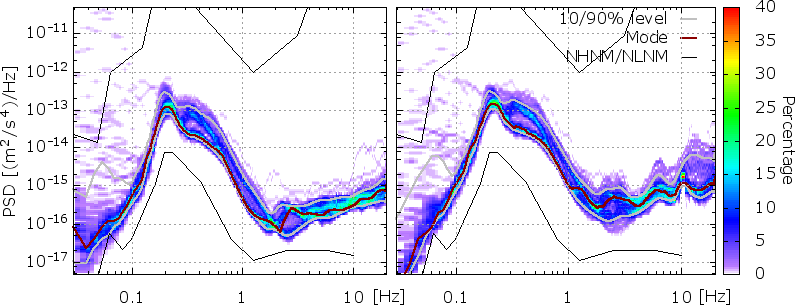
\includegraphics[width=\textwidth]{./Sec_SiteInfra/Figures/results/Canfranc-B_multiplot1}
\caption{The horizontal component (left) and the vertical component (right) power spectral density plotted as a spectral variation from the Spain - Laboratorio Subterr\'eneo de Canfranc site.}
\label{fig:Canfranc-B_multiplot1}
\end{figure}\begin{figure}[h]
\centering
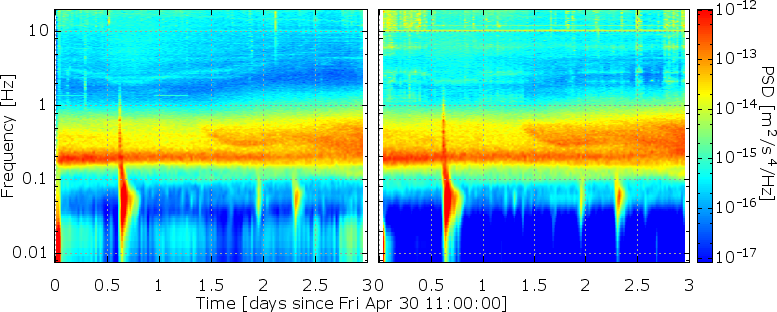
\includegraphics[width=\textwidth]{./Sec_SiteInfra/Figures/results/Canfranc-B_multiplot2}
\caption{The spectrogram of the horizontal (left) and vertical (right) component from the Spain - Laboratorio Subterráneo de Canfranc site.}
\label{fig:Canfranc-B_multiplot2}
\end{figure}

\pagebreak
\FloatBarrier
\subsubsection*{Finland - Sumiainen}
\begin{figure}[h]
\centering
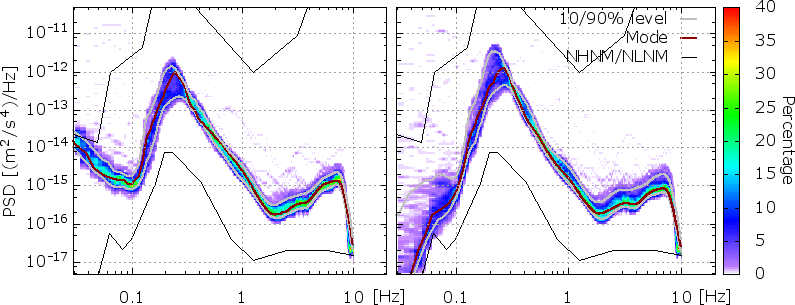
\includegraphics[width=\textwidth]{./Sec_SiteInfra/Figures/results/SUF_multiplot1}
\caption{The horizontal component (left) and the vertical component (right) power spectral density plotted as a spectral variation from the Finland - Sumiainen site.}
\label{fig:_Finl_multiplot1}
\end{figure}\begin{figure}[h]
\centering
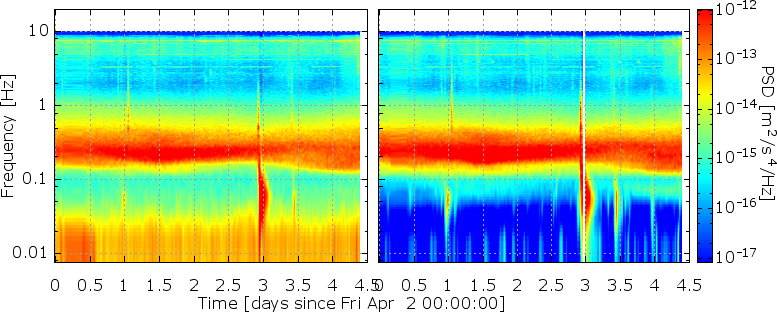
\includegraphics[width=\textwidth]{./Sec_SiteInfra/Figures/results/SUF_multiplot2}
\caption{The spectrogram of the horizontal (left) and vertical (right) component from the Finland - Sumiainen site.}
\label{fig:_Finl_multiplot2}
\end{figure}

\pagebreak
\FloatBarrier
\subsubsection*{France - Frejus}
\begin{figure}[h]
\centering
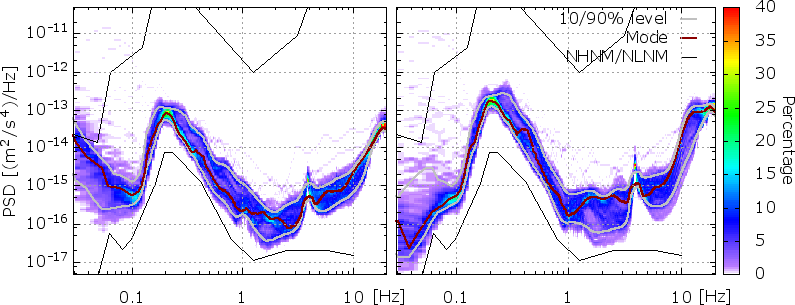
\includegraphics[width=\textwidth]{./Sec_SiteInfra/Figures/results/Frejus-A_multiplot1}
\caption{The horizontal component (left) and the vertical component (right) power spectral density plotted as a spectral variation from the France - Frejus site.}
\label{fig:Frejus-A_multiplot1}
\end{figure}\begin{figure}[h]
\centering
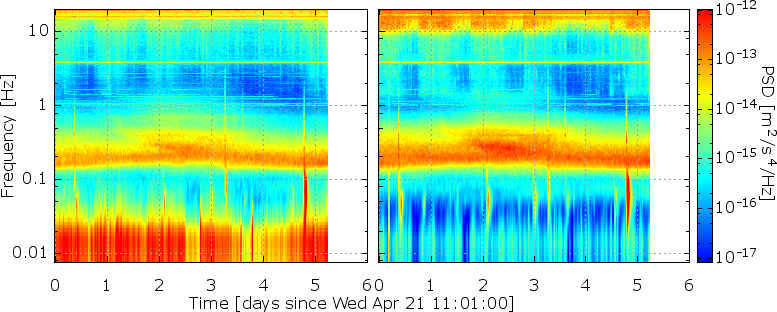
\includegraphics[width=\textwidth]{./Sec_SiteInfra/Figures/results/Frejus-A_multiplot2}
\caption{The spectrogram of the horizontal (left) and vertical (right) component from the France - Frejus site.}
\label{fig:Frejus-A_multiplot2}
\end{figure}

\pagebreak
\FloatBarrier
\subsubsection*{Italy - Gran Sasso}
\begin{figure}[h]
\centering
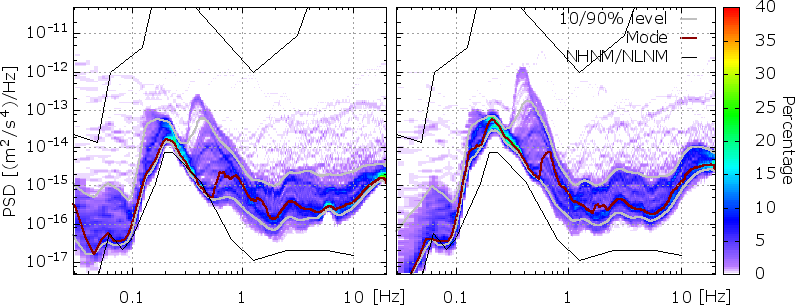
\includegraphics[width=\textwidth]{./Sec_SiteInfra/Figures/results/GSasso-A_multiplot1}
\caption{The horizontal component (left) and the vertical component (right) power spectral density plotted as a spectral variation from the Italy - Gran Sasso site.}
\label{fig:GSasso-A_multiplot1}
\end{figure}\begin{figure}[h]
\centering
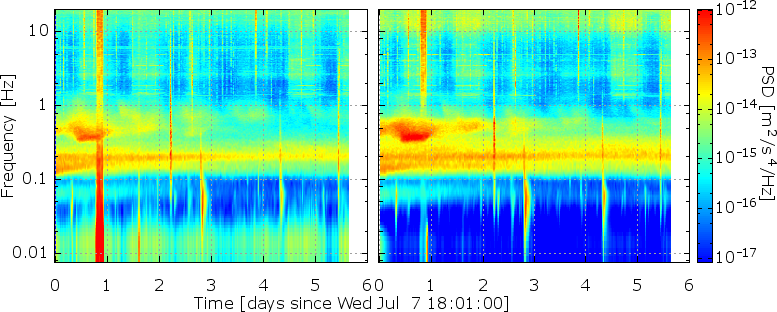
\includegraphics[width=\textwidth]{./Sec_SiteInfra/Figures/results/GSasso-A_multiplot2}
\caption{The spectrogram of the horizontal (left) and vertical (right) component from the Italy - Gran Sasso site.}
\label{fig:GSasso-A_multiplot2}
\end{figure}

\pagebreak
\FloatBarrier
\subsubsection*{Japan - Kamioka mine}
\begin{figure}[h]
\centering
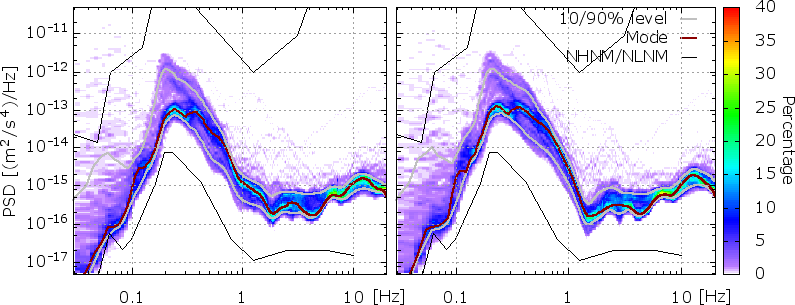
\includegraphics[width=\textwidth]{./Sec_SiteInfra/Figures/results/Kamioka-A_multiplot1}
\caption{The horizontal component (left) and the vertical component (right) power spectral density plotted as a spectral variation from the Japan - Kamioka mine site.}
\label{fig:Kamioka-A_multiplot1}
\end{figure}\begin{figure}[h]
\centering
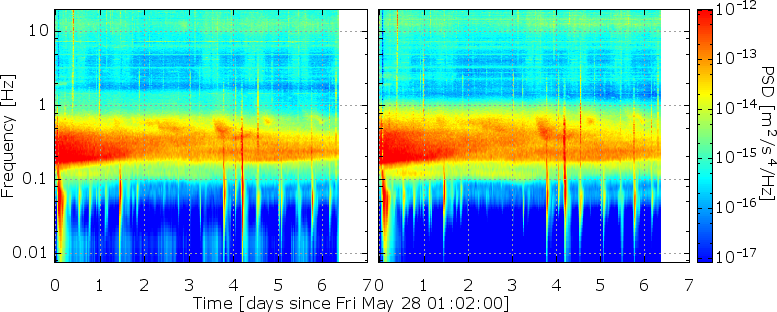
\includegraphics[width=\textwidth]{./Sec_SiteInfra/Figures/results/Kamioka-A_multiplot2}
\caption{The spectrogram of the horizontal (left) and vertical (right) component from the Japan - Kamioka mine site.}
\label{fig:Kamioka-A_multiplot2}
\end{figure}

\pagebreak
\FloatBarrier
\subsubsection*{Germany - Moxa}
\begin{figure}[h]
\centering
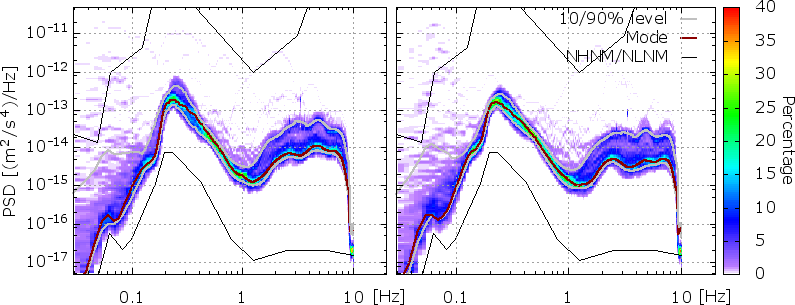
\includegraphics[width=\textwidth]{./Sec_SiteInfra/Figures/results/MOX_multiplot1}
\caption{The horizontal component (left) and the vertical component (right) power spectral density plotted as a spectral variation from the Germany - Moxa site.}
\label{fig:_Moxa_multiplot1}
\end{figure}\begin{figure}[h]
\centering
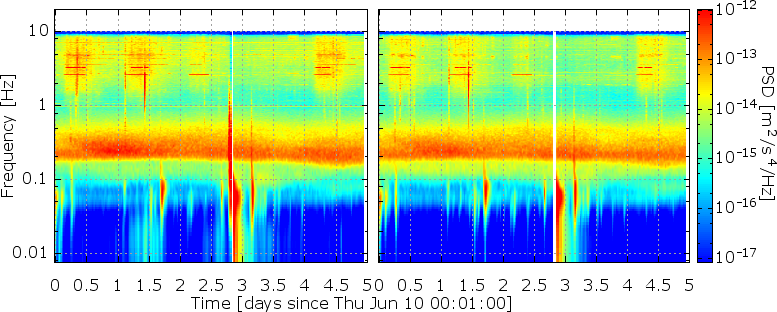
\includegraphics[width=\textwidth]{./Sec_SiteInfra/Figures/results/MOX_multiplot2}
\caption{The spectrogram of the horizontal (left) and vertical (right) component from the Germany - Moxa site.}
\label{fig:_Moxa_multiplot2}
\end{figure}

\pagebreak
\FloatBarrier
\subsubsection*{Netherlands - Heimansgroeve}
\begin{figure}[h]
\centering
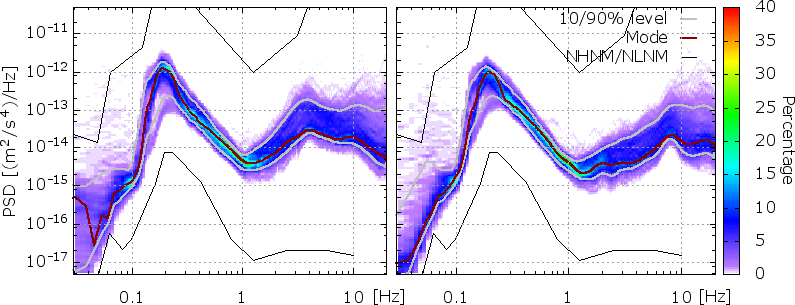
\includegraphics[width=\textwidth]{./Sec_SiteInfra/Figures/results/Heimans-A_multiplot1}
\caption{The horizontal component (left) and the vertical component (right) power spectral density plotted as a spectral variation from the Netherlands - Heimansgroeve site.}
\label{fig:Heimans-A_multiplot1}
\end{figure}\begin{figure}[h]
\centering
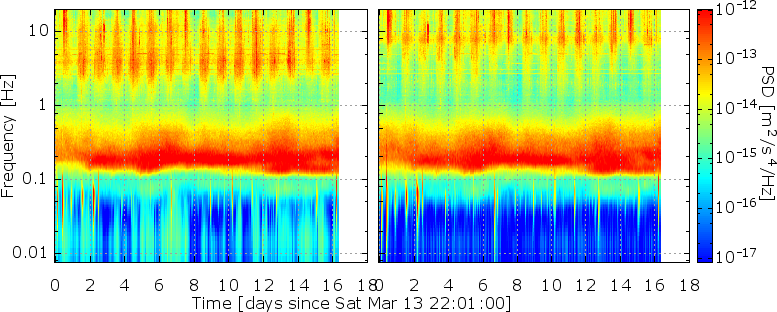
\includegraphics[width=\textwidth]{./Sec_SiteInfra/Figures/results/Heimans-A_multiplot2}
\caption{The spectrogram of the horizontal (left) and vertical (right) component from the Netherlands - Heimansgroeve site.}
\label{fig:Heimans-A_multiplot2}
\end{figure}

\pagebreak
\FloatBarrier
\subsubsection*{Romania - Slanic-Prahova}
\begin{figure}[h]
\centering
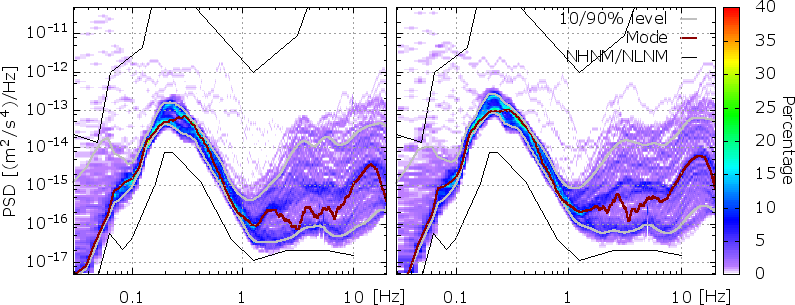
\includegraphics[width=\textwidth]{./Sec_SiteInfra/Figures/results/Slanic-A_multiplot1}
\caption{The horizontal component (left) and the vertical component (right) power spectral density plotted as a spectral variation from the Romania - Slanic-Prahova site.}
\label{fig:Slanic-A_multiplot1}
\end{figure}\begin{figure}[h]
\centering
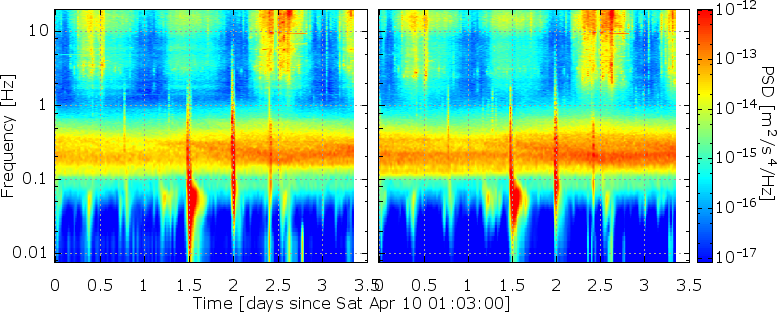
\includegraphics[width=\textwidth]{./Sec_SiteInfra/Figures/results/Slanic-A_multiplot2}
\caption{The spectrogram of the horizontal (left) and vertical (right) component from the Romania - Slanic-Prahova site.}
\label{fig:Slanic-A_multiplot2}
\end{figure}

\pagebreak
\FloatBarrier
\subsubsection*{Belgium - Mol}
\begin{figure}[h]
\centering
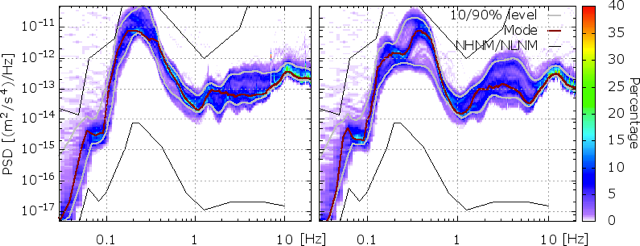
\includegraphics[width=\textwidth]{./Sec_SiteInfra/Figures/results/Mol-A_multiplot1}
\caption{The horizontal component (left) and the vertical component (right) power spectral density plotted as a spectral variation from the Romania - Slanic-Prahova site.}
\label{fig:Mol-A_multiplot1}
\end{figure}\begin{figure}[h]
\centering
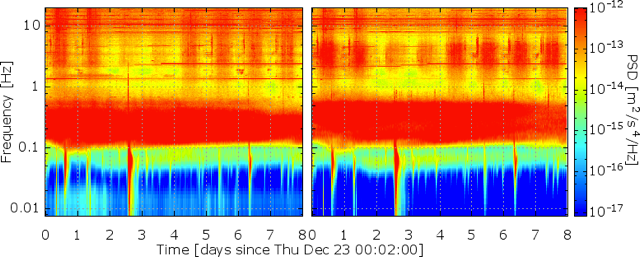
\includegraphics[width=\textwidth]{./Sec_SiteInfra/Figures/results/Mol-A_multiplot2}
\caption{The spectrogram of the horizontal (left) and vertical (right) component from the Romania - Slanic-Prahova site.}
\label{fig:Mol-A_multiplot2}
\end{figure}
\FloatBarrier
%\subsection{Appendix B: ET infrastructure drawings}
